\subsubsection{Strat ME}

\paragraph{Outline}

Are there dominating FTBs that come with t1/t2 contact? Pick them. If not find best bonuses and regions in the board and setup picks in a way that will give you an advantage in any way (more income, more armies, a double border, a stack, positional, safe income whatever) on a specific turn.

3x4, neutrals 2/4, wastelands 7/10, base +5

\paragraph{Map Dynamics}

Well the map has been studied extensively, so a lot of things I list here are a repetition. 

\begin{figure}[H]
  \centering
  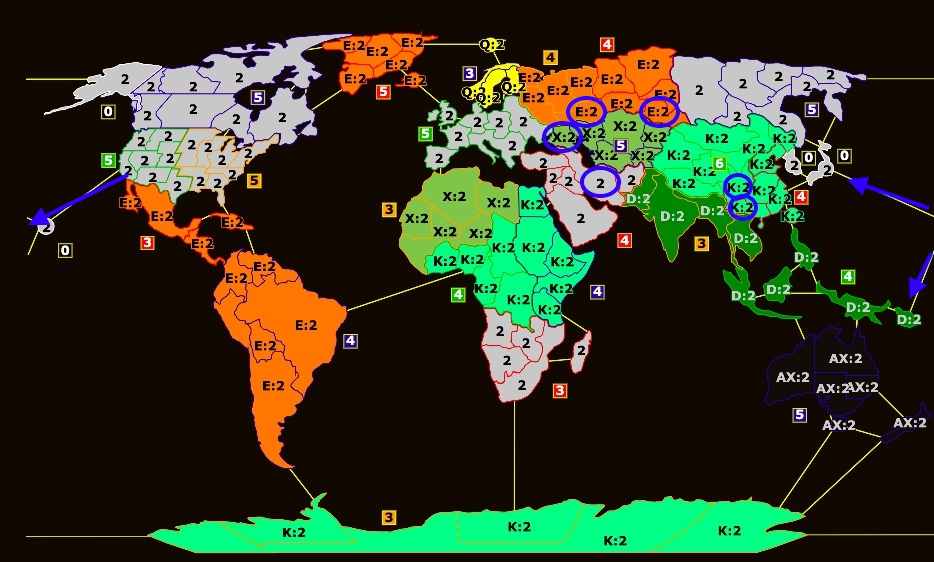
\includegraphics[width=0.9\textwidth]{Images/strat_me_dynamics.jpg}
  \caption{Bonus Win-Rates for Games with Overall Winner Rating >=1800 in Strat ME(n=354) (AX>D>K>Q>E>-), with important bottlenecks.}
  \label{strat_me_dynamics}
\end{figure}

Diving into Figure \ref{strat_me_dynamics}:
\begin{enumerate}
    \item AX: >60\% WR.
    \begin{itemize}
        \item Europe and Australia have 70\% and 68\% WR. I'm not including EU in the map due to it having 12W in 17G, it's practically a counter pick with like 2-3 exceptions, \href{https://www.warzone.com/MultiPlayer?GameID=40719588}{here} from Forsaken in CL18 as a triple pick (similar idea \href{https://www.warzone.com/MultiPlayer?GameID=38606079}{here}), \href{https://www.warzone.com/MultiPlayer?GameID=22938461}{here} from Rufus as an actual bonus, \href{https://www.warzone.com/MultiPlayer?GameID=37057617}{here} by Juan to combo UK + Greenland in order to counter Scandi (didn't work but that's the idea). Besides above niche and innovative applications that can work, it's really just a Scandi + Europe ftb angle. \href{https://www.warzone.com/MultiPlayer?GameID=32635176}{Gak vs Kage}, \href{https://www.warzone.com/MultiPlayer?GameID=32490164}{same} or as a counter pick to that very ftb like \href{https://www.warzone.com/MultiPlayer?GameID=18397489}{here} by both players. 
        \item Australia is a spectacular bonus in that:
        \begin{enumerate}
            \item Combo +5 with 1 double border, very safe, 2 turns away from Asia
            \item Incredibly fast expansion in Indonesia, the 2nd best bonus. \href{https://www.warzone.com/MultiPlayer?GameID=37030485}{example}
            \item Can defend itself with a blockade from Antarctica very easily by baiting resources. (Goes both ways). For example \href{https://www.warzone.com/MultiPlayer?GameID=33924215 }{here}, \href{https://www.warzone.com/MultiPlayer?GameID=37434686}{here}
            \item ftb with Antarctica. example \href{https://www.warzone.com/MultiPlayer?GameID=36889391}{here}
        \end{enumerate}
    \end{itemize}
    \item D: >55\% WR. SEA, Indonesia. the latter, follows the same principles with Australia. Single borders -> easy to defend. Great expansion. Pathway within 2 turns to major income regions in West US/CA and WC. Can stop expansion from Antarctica. SEA is a versatile bonusas it is 2 turns away from breaking every single bonus in Eurasia. You'll find in your games that SEA not only is really hard to break, but also gives you flexibility when dropping it, as it is even harder for your opponent to eliminate you.
    \begin{itemize}
        \item In SEA vs Scandinavia or SEA vs WR/CR boards, as the SEA player you have pathways from Iran and Caucasus into breaking those bonuses. Simple plan of build a stack -> kill. this extends to the overall downside that region of Scandi/WR/CR have in that they are easy to break. \href{https://www.warzone.com/MultiPlayer?GameID=40511685}{Here} Octane is down 8 Income but has a simple plan in getting in there and punching with a stack. So coming back to the SEA vs Scandi/WR/CR argument:
        \begin{enumerate}
            \item you build stack Iran->Georgia-> Break WR.
            \item they build stack Xinjiang -> Pakistan and Break SEA
        \end{enumerate}
        \item After the break, if you had SEA + Indonesia they are 4 turns away, if you had SEA + somewhere else on the map, they have a bunch of useless armies in Pakistan and will never eliminate you for the bonus is a straight line. Your stack is in a better position. For example \href{https://www.warzone.com/MultiPlayer?GameID=20536396}{here}, as much as Rufus broke SEA, it is impossible to move towards Indonesia. A couple of turns later, Rufus breaks Indonesia from Hawaii, but those armies are again misplaced and this gives just enough tempo for Njord to pivot. 
    \end{itemize}
    \item K: >50\% WR. Africa bonuses, Antarctica, WC, EC. All of these come in different conversations.
    \begin{itemize}
        \item On Antarctica and Asia, Antarctica is an incredible bonus, absolutely fascinating. Can combo with Aus/SA for +4 or +5 in 2 turns. Has single borders -> easy to defend, has an entrance to Africa, and can be flexible in baiting resources. It is a slow bonus, that is all. In some distributions you have to realize there are better options than just a very safe remote +3 bonus. For example, \href{https://www.warzone.com/MultiPlayer?GameID=21060202}{here} Njord simply triple picks Asia. If you get tomsk and Iran it is so easy to defend despite the fact Aura has, in theory, safer income. In contrast \href{https://www.warzone.com/MultiPlayer?GameID=40072623}{here}, I make it in time just barely and Beep misplayed sending useless armies to Indonesia instead of securing Asia. this gives me a great pass to discuss the Asia bonuses. EC is a great single +4 safe bonus and WC can both be a counter, a double pick with SEA/WC/EC and a triple pick. 
        \item Africa is conflicted. Can be really god. Can be god awful.
    \end{itemize}
    \item X have high WR but are mainly counter-picks
    \item Q: Scandinavia at 50\% exactly as well as E: >43\% WR. 
    \begin{itemize}
        \item Starting with Scandinavia, it is a great pick, just slightly over-picked from people not wanting to calculate the position more than 2 turns in. Scandinavia in general shines if it can reach Ufa with a stack and break CR, or has expansion in either of WR/EU/Greenland. If you don't reach Ufa like \href{https://www.warzone.com/MultiPlayer?GameID=34547862}{here}, game's lost.
        \begin{itemize}
            \item Combos with Greenland for combo +5 \href{https://www.warzone.com/MultiPlayer?GameID=38946241}{here} and \href{https://www.warzone.com/MultiPlayer?GameID=40572104}{here} and \href{https://www.warzone.com/MultiPlayer?GameID=34052341}{here}. Incredibly powerful but 1st pick dependent. Pay attention to how the players expand using a 3attack from Svalbard, so in case it doesn't work, you can recapture next turn (usually without deploying. WR 101).
            \item Combos with Greenland for ftb. \href{https://www.warzone.com/MultiPlayer?GameID=37573271}{example}, \href{https://www.warzone.com/MultiPlayer?GameID=33048983}{failed example}, \href{https://www.warzone.com/MultiPlayer?GameID=32584403}{weird example of how to not pick your 5} and so on.
            \item More niche combos like \href{https://www.warzone.com/MultiPlayer?GameID=33613524}{here} and \href{https://www.warzone.com/MultiPlayer?GameID=29179449}{here} for slower income transition. 
            \item Key difference between the above 3 categories is \textbf{timing}, something extremely important in every template and especially modified earth ones. If you pick ftb you want to fight t1/t2. If you pick a combo +5 with a counter you want some configuration going into a double border on t3/t4 (often), but generally want to avoid contact earlier. If you pick for slower income as above (16/17/18) by end of turn 4, you dont want contact up to turn 5, and a position that will counter your opponent's expansion on t5/t6. 
        \end{itemize}
        \item CA and SA are very popular picks for straight forward reasons. In a handful of distributions you can check the board and within 1 second do 1/2 SA, CA 3456 Asia in some contested rich-in-income region. Sadly, this can work, it is a strategy that revolves around getting to 9 income and playing the 9v8 or 9v9 or 9v11 income game with safe income. Simple example in \href{https://www.warzone.com/MultiPlayer?GameID=37304447}{this game}, where tornado does 3456 an EC ftb with 4 spawns. Another example \href{https://www.warzone.com/MultiPlayer?GameID=33517812}{here}, with both players committing the the 1/2 SA and 3456 Asia combos. At the same time these bonuses, individually, are really strong and a tiny bit overrated.
        \begin{itemize}
            \item CA shines as an ftb. For example \href{https://www.warzone.com/MultiPlayer?GameID=33091886}{here} Rufus' idea on picks is straight-forward. Pick ftb, 3/4 neighbouring territories -> fight and eliminate. Another example \href{https://www.warzone.com/MultiPlayer?GameID=20536396}{here} with a different configuration of ftb CA and asia combos. In these setups generally the game is all about tricks, card pieces and above all army advantage, as that is something that can be converted into an advantage and later a win.
            \item SA combos with many different bonuses and provides in general a safe +4 bonus with nice proximity. that said it can be slow if you don't get contact the turn after completing, or ifyou don't have information. For example in SA/CA vs EAf setups, if you don't know of Eaf and they hit Nigeria with a stack when you are expanding through Antarctica or Hawaii, say bye to +8 Income.
            \item WR/CR are very easy to complete and in an income rich region, that is however very accessible. Scandi vs CR, whoever gets Ufa wins. WR vs WC/EC, if you get to tomsk you can win, if not press the red button.
        \end{itemize}
        

    \end{itemize}
\end{enumerate}

\paragraph{Picking Logic}

Repeating something I said in a previous section, Strat ME is a lot about timing, and then building an army advantage. timing of contact comes in effect in picking, as you want to find a configuration that allows you to have more income/armies on a better position at a turn of choice. 
\\
\\
that said, 7/10 strat me games are about specific combos that are extremely strong and you have to cover on 1/2 or 1/3. this dictates the way you'll order your later picks. For sake of simplification let's say you always 1/2 the bonus. (1/3 is in situations like Svaalbard/Nuuk spawns in Greenland/Scandi where your 3rd pick is so useless without first, though still pick combinations are the same, you can get 1/2/5 or 1/3/5 and so on. Real difference comes when your opponent doesn't have the same first pick. In such a scenario, if he is FP, you get 1/2 combo Greenland, and not 1/3. In this template specifically this matters less since its RMO. In MME you could argue that getting 1/3 and suspecting your opponent first-picked your 2 hints at him being first pick. Whatever.)
\begin{itemize}
    \item 1/2 ftb CA/Ant/SEA you want to look for immediate contact or contact turn 2/3. Use the Income advantage to your benefit.
    \item 1/2 +4 bonus secures it's completion. Solo pick +4 is a 96\% gamble (bomb of strategicness). Combo +4 and counter t3 with a 4 attack or t4 with a stack works in your favor. Stuff like CA/SA/WR spawn, get SA in two, move to Ufa with 4 armies end of turn 2, 9vs9 income vs a completed CR and all in. Later picks can be neighboring or not. 
    \begin{itemize}
        \item Setups like 1/2 CA, SA, 3/4 another combo 5/6 another combo, where 1/3/4 gives you a safe +4 and a fight on 1/2. 
        \item Or setups like 1/2 CA, SA, 3/4/5 region coverage 6 counter pick or single pick, 
        \item or 1/2 combo, 3 single pick, 4/5/6 cover. 
        \item All these are both a matter of perspective, play-style, and flexibility. 4/5/6 coverage with 3 safe single pick always risks getting 1/2/3 and losing to a triple pick. It also generally speaking puts 1st pick at a great disadvantage, as if you full mirror 1/4/5 will lose to 2/3/6 due to FP having 3 contested picks and SP having 2 contested picks. But nothing is absolute, all depends on your distribution.
    \end{itemize}
    \item Combo +5 for safety requires contact a bit later. 
    \item In the other 3/10 distributions you can't find combos that govern income regions and demand priority, so single picks (or even triple picks for WC/EC/SEA, or EU/Greenland/Scandi and triple Africa but very rare) arise, slower income comes in play, mme style. typically 12-14 income by end of turn 3 (+4 and +5 bonuses for 14, +4 and +4 for 13 etc), or 16-18 income by end of turn 4 (+5/+5/+3 for 18, +5/+4/+3 for 17 etc). Slower income transition -> Remote bonuses that you can complete safely and setup contact later, either on the rf t5 turn or even later in the bonuses your opponents will expand at.
\end{itemize}


\paragraph{Gameplay}
% early, mid, cards

Strat ME has been one of the most popular templates, as a) it was the old 1vs1 ladder b) it's been featured twice as the seasonal ladder \href{https://www.warzone.com/LadderSeason?ID=4069}{Season 38} and \href{https://www.warzone.com/LadderSeason?ID=4020}{Season 21} c) it has been selected in multiple strat competitions (\href{https://www.warzone.com/MultiPlayer/Tournament?ID=56704}{AWP 2024}, \href{https://www.warzone.com/MultiPlayer/Tournament?ID=51304}{AWP 2023}, \href{https://www.warzone.com/MultiPlayer/Tournament?ID=47859}{AWP 2022} (\textit{can find more in the AWP 2016-2021 sheet}), \href{https://docs.google.com/spreadsheets/d/1xk1MMZo14ujGI823fZLqzK6_4j00x8YZf4GnK_8dvVA/edit?usp=sharing}{ML3}, \href{https://docs.google.com/spreadsheets/d/1-CXBKQ8pDioH2Cu6dKtZlO9qlyReanwGysu27a1D590/edit?gid=19021413#gid=19021413}{CL 18}, \href{https://docs.google.com/spreadsheets/d/1oVI29Qupn9jqAZ1eBbzvewCjzlDTZZsdBkYLAOy6crs/edit}{CL 16}, \href{https://docs.google.com/spreadsheets/d/1-M-IGtNTlpuVhHO4RlQQjEIEDUF-5ln91xQH5DB6Pwk/edit?gid=323930043#gid=323930043}{CL 14} and more. It is quite possibly the tested, studied and thoroughly discussed template. On top, most of the pre-existing guides, like GG's guide, are about that map and settings.
\\
\\
From my experience Strat ME is the best template to experiment, apply and understand a lot of WR tricks and methodology around expansion and gameplay. When ahead, the game is about converting that lead/advantage into something of substance. An elimination, a big army advantage, a bonus capture, etc. When behind, the game is about playing for your win conditions even if that includes the most lunatic random strategies existing. And to be honest, this is my main advice for this template, as in understand what needs to be done for you to win the game and do it, regardless of it's nature.
\\
\\
First example in a recent game for me \href{https://www.warzone.com/MultiPlayer?GameID=41475154}{vs Octane}. the board has roughly 3 regions, SA, Europe and Asia and the easiest way to simplify the board is 1/2 SA into 3456 Eurasia. Getting 1/2 guarantees safe income and a coverage spawn. Splitting 1/2 comes with early fights and contest in multiple fronts. I was conflicted on these sets, if you can follow my logic or if it makes sense in the first place. I can see sets like the one above, that follow either of the 3 paths: 
\begin{itemize}
    \item a) 1/2 SA 3 EC 4/5 CR WR 6 Scandi.
    \item b) 1/2 SA 3 Scandi 4/5 WR, CR, 6 ER.
    \item c) the set Octane went for, 1/2 SA, 3/4 CR, WR, 5 Scandi, 6 EC.
\end{itemize}

Besides these sets, there's some more niche strategies, as following:
\begin{itemize}
    \item d)1/2/3 Europe CR/WR/Scandi 4/5 Ant Sa 6 Waf (or Australia).
    \item my set of 1 Scandi 2/3 SEA/Indo 456 SA, Ant Waf.
\end{itemize}

At this point, before going in depth to all 16 configurations between sets a-d, ask yourself what outcome do you want to get 1,2, 3 turns in the game so as to convert it to a win. From Octane's POV, you sort of expect mirroring 1/2, pick CR in case you get 123 to threaten both EU and EC as well as hope for a positive outcome as 2nd pick with 234 and combo EC. From my POV, I pick planning to get either of the following. 123, 136-135 or 236. 123 I do what I did in the game, rush to Ufa with stack which perfectly aligns with the rf card on turn 5, break, and have Indonesia to counter SA/Ant expansion into Aus. 135 and similar sets are pretty wild but possible, as they have Octane picking EC/SEA combo and either of SA and Ant. I have Scandi into Indo completion on turn 3 into blast SEA turn 4 with +12, which is ok. 236 is the ideal outcome. My set isn't foolproof but it is unexpected, which can both be good and bad. It's bad because I'm deviating from the best picks and a good player will punish me. It can be good because my opponent might waste resources in the wrong region due to having to guess. Ask 50 good WR players and I can guarantee you at bare minimum 45 will pick SA combo. 
\\
\\
this is where my motto in WR surfaces. "Find the line that can either get you back in the game or convert the advantage, and either lose trying or win doing so". I picked this way planning to breaking on turn 5 CR and knowing I'm playing against CR/SA/Ant or WR/SA/Ant (vs the latter the game is easier for me). I can't deviate and if I fail t5 breaking, I lose, surrender turn 5, gg wp. My pick-set is fundamentally flawed when it relies on such a coin-flip, albeit it's part of the game. By turn 6, the game is 12vs12 income, and somewhat equal armies on the field. It is now a chicken game, where we both stack armies, hope the other person makes a mistake, play mind-games, and stall. 

\begin{figure}[H]
  \centering
  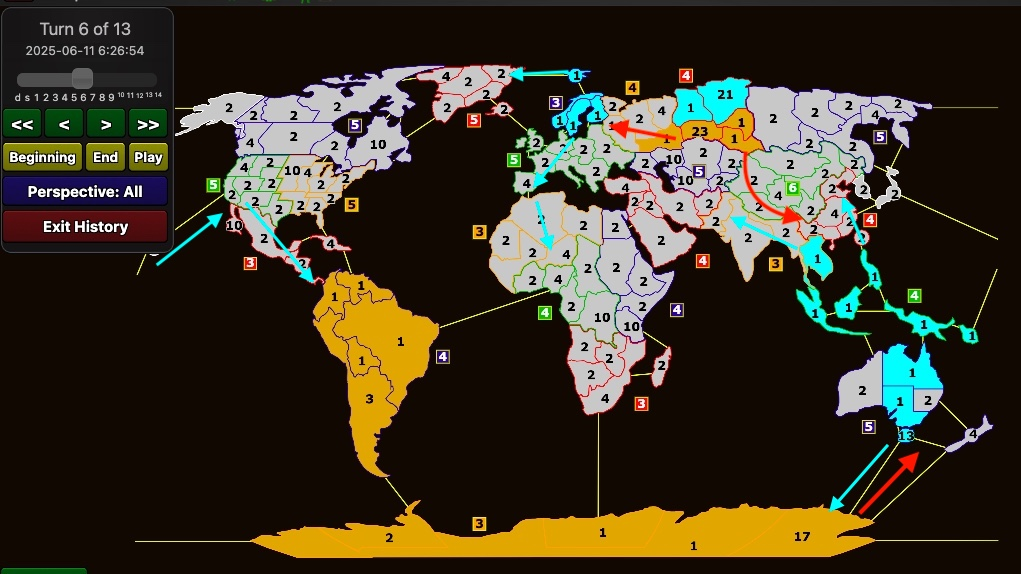
\includegraphics[width=0.9\textwidth]{Images/gameplay_op.jpg}
  \caption{Position in Strat ME and options}
  \label{strat_me_gameplay}
\end{figure}

Positionally, taking into account Figure \ref{strat_me_gameplay}, you need to evaluate the position and ask yourself what's the best course of action for both players. I'm in an equal income -6 armies position, where I hang by an edge but threaten a lot. Octane is stuck in a corner and has to take an initiative or react (early or late) to something I plan.
\begin{itemize}
    \item My ideas are as following:
    \begin{enumerate}
        \item Expand towards SA fom EU and get bonus, very slow, octane will get an enormous army advantage elsewhere in the meantime and pivot there, either CR and region or Aus/Indo.
        \item Expand in Greenland which is slow, but safe. It can sort of work though. Reason is I can also expand in SEA or EC, the natural options, which Octane can cover with 3 turns easily. I would undoubtedly lose Aus there though, same for SAf, and maybe even CR.
        \item Start a journey to CA which you can do but would have to abandon Aus.
        \item Start faking everything, hiding deployments and hoping for the best.
    \end{enumerate}
    \item For Octane, he absolutely has to all in me one of the following turns to get an army advantage, there isn't any other way to convert an advantage. Ideally he all in's Tasmania twice in a row and snowballs the game from that army advantage. If he can't figure out what I'm doing, it gets tricky. If I expand in Greenland, drop Aus and he thinks I'm in EC/SEA, I'll get a tempo edge as he will have armies wasted in Asia. If I expand in SEA/EC and he spots it I'm lost. But if I expand in Greenland and he doesn't fall the bait he can eliminate CR, Aus, or both. Play-style comes in place here.
\end{itemize}

My idea is that here expanding mindlessly is most certainly a loss and the only course of action is muddying the waters and take advantage of the fact Octane has to react to ghosts. As such, on turn 7 I full deploy drop back to salvage army loses and get 1 turn tempo lead in a distance of a territory between us. that way turn 8 he cannot attack my stack. turn 8 I minimize losses in CR, stay idle in an important territory, and deploy behind the fog, baiting SEA/EC. turn 9 I have to react to the army disadvantage in CR and must fall for the bait. If I don't and get wiped it's tough, but I leave my options open, transition towards WR, secure my stack, and let him expand. He has to react to SEA/EC/Greenland and SAf + counters are the course of action. 
\\
\\
Miracle number 2, turn 10, I get the RMO coinflip and now the position is winning for me (\textit{Even if I lost the RMO flip, I get a spectacular trade, just not as good}). My maneuver from t7 in getting a tempo win to save my stack up to t10 to get a favorable trade was precisely for this moment. If he doesn't overextend there I will build a stack and break Antarctica even if I have to deploy 50 armies for it, for he already chose to move towards SEA/EC, and I can get card pieces now in WR to match his SAf (and Australia).
\\
\\
the game now isn't anymore about making a comeback, but it is about converting the advantage, so the plan changes. Gamble Australia which is harmless because if he counters, I will use one of the 2 territories in Tasmania and New Zealand, to break Antarctica. Complete CR, maybe even EU, let him come to SEA/Indo. 
\\
\\
Miracle number 3, out-delay and guess the right territory on turn 12 (I misplayed, should've secured out-delaying, but god showed mercy). 
\\
\\
My point at the end of the day, is that if you pick recklessly or generally get into tough positions where if you do something you'll slowly lose positionally, find your win conditions. For me it all started with acknowledging I picked like a clown and the game is unplayable if I don't succeed in the turn 5 flip, followed by the mind-games, tempo swing on t7 and army advantage push between t7-t10.
\\
\\
\textbf{Other examples from CL and other competitions}.

In short tips:
\begin{enumerate}
    \item \href{https://www.warzone.com/MultiPlayer?GameID=33909207}{CL16 Octane/adrenaline}. It's an 8vs8 income game with 2 different fronts -> the game is all about the balance between army advantage and card pieces. By t4, Octane takes the L in Africa, tries to get any army adv he can get in NA on t5 and keeps rf to salvage the army disadvantage later whenever it's needed. It is very hard for both players to sneak a bonus without losing a front. take note of the positional play in securing a safe region, building a stack, surviving and only breaking when your opponent has already overextended defending. 
    \item \href{https://www.warzone.com/MultiPlayer?GameID=40954287}{CL18 Jacob/Forsaken}. take note of all the tempo swings and attempts at getting small advantages over the board.
    \begin{itemize}
        \item Forsaken blockades Scandi on turn 5 keeping a spawn alive in order to survive in Eur-Asia and acknowledging his win condition is building a stack and getting into Asia and Oceania, pivoting to a CA/Waf/West US and potentially Saf game.
        \item Jacob has to drop Indonesia and block the entrance to Aus as that keeps his position hidden and makes forsaken think he has Aus. He has wasted armies in Greenland so he has to pivot to Scandi, must cover West US, and pivot into CR after losing Indonesia, as it is now the safest bonus. 
        \item By turn 8 the game is a counting mess because Forsaken is faking West US, has Germany/Sweden to threaten 2 entrances to Greenland, and is moving towards SEA double border. the game now is about positioning armies into important territories -> Useful armies.
        \item From here onwards every single move is just a pain to see. a)t9/t/10 Forsaken gets army advantage and threatens everywhere. Jacob has to play passive. He has income advantage, needs to get army advantage from the 14vs12 position. Cannot Lose Scandi, not drop West US without something in return. b) Forsaken t11 slips overextending, but gets great trades on t12 and survives in UK just to threaten with 3 armies. c) Jacob's 2 extra armies in SEA buy him just enough time, along with Forsaken playing it safe. and not sending the whole stack towards Pakistan. Imagine the position end of turn 15 if Forsaken captures with stack India. the small tempo swing buys time for Jacob to threaten Canada and rebuild stacks in Greenland/Scandi. By the time Forsaken figures out CR -> evacuate -> clear Canada borders -> pivot, and push forward Scandi. Defending Ufa double border is a nightmare and will not work, be proactive. Forsaken sees through it and threatens Canada on turn 18. Cannot pivot to anything else anymore and cannot drop West US and Canada -> accept the game is now a a defensive coinflip -> play it out and either come victorious or lose.
    \end{itemize}
\end{enumerate}

